%!TEX program = xelatex
%%%%%%%%%%%%%%%%%%%%%%%这是导言部分的开始%%%%%%%%

%========= 导言部分声明文档的类型=================
\documentclass{article}

%=========导言部分可可以加载宏包=================
\usepackage{amsmath}                % 数学公式排版宏包
\usepackage{amssymb}                % 数学符号命令宏包
\usepackage{amsthm}                 % 数学定理宏包
\usepackage[UTF8]{ctex}             % 中文输入宏包
\usepackage[a4paper]{geometry}      % 页面设置宏包
\usepackage{setspace}               % 行间距宏包
\usepackage{graphicx}               % 图片宏包
\usepackage{listings}               % 代码宏包
\usepackage{color}					% 颜色宏包
\usepackage{xcolor}                 % 颜色处理宏包
\usepackage{float}                  % 浮动对象式样宏包
\usepackage{fontspec}
\usepackage{enumerate}				% 列举编号包

%=========页面设置==============================
\geometry{left=1cm,right=1cm,top=1cm,bottom=2cm}
\onehalfspacing
\setlength\parindent{0em}

%=========代码格式设置============================
\definecolor{dkgreen}{rgb}{0,0.6,0}
\definecolor{gray}{rgb}{0.5,0.5,0.5}
\definecolor{mauve}{rgb}{0.58,0,0.82}
% \setmonofont{Consolas}
\lstset{
	numbers = left, 	
	numberstyle = \color{gray}, 
	keywordstyle = \color{blue},
	commentstyle = \color{dkgreen}, 
	stringstyle = \color{mauve},
	basicstyle = \ttfamily,
	breaklines = true,
	frame = shadowbox, % 阴影效果
	rulesepcolor = \color{ red!20!green!20!blue!20} ,
	escapeinside = ``, % 英文分号中可写入中文
	xleftmargin = 2em,xrightmargin=2em, aboveskip=1em,
	framexleftmargin = 2em
} 

%=========导言部分可以定义标题信息===============
\title{组会报告}
\author{徐益}
\date{\today}
%%%%%%%%%%%%%%%%%%%%%%%这是导言部分的结束%%%%%%%%%

%%%%%%%%%%%%%%%%%%%%%%%这是正文部分的开始%%%%%%%%%
\begin{document}

%=========生成标题================================
\maketitle

%=========开始正文的输入==========================

%===========第一节=================
\section{工作内容} 
1. 修改NR单线程链路中的问题;

2. 性能测试。

%===========第一节=================
\section{NR单线程链路问题修复}
\subsection{流不满时的信道估计问题}
\begin{figure}[H]
	\centering
	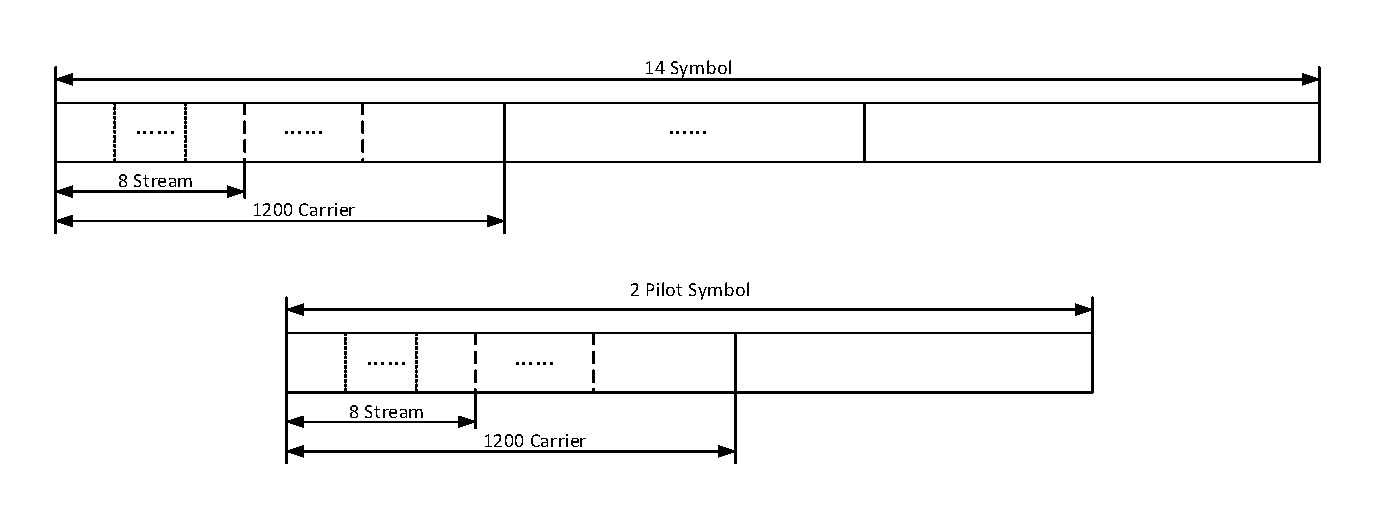
\includegraphics[width = \textwidth]{data.pdf}
	\caption{Tx端数据子帧结构}
\end{figure}
\subsubsection{方案一:截取满流(8 Stream)时的导频}
问题:\\
1. 信号估计前需要对导频进行截取,增加开销\\
2. 低流时无法使用更密集的导频\\
\begin{figure}[H]
	\begin{minipage}[t]{0.5\linewidth}
	\centering
	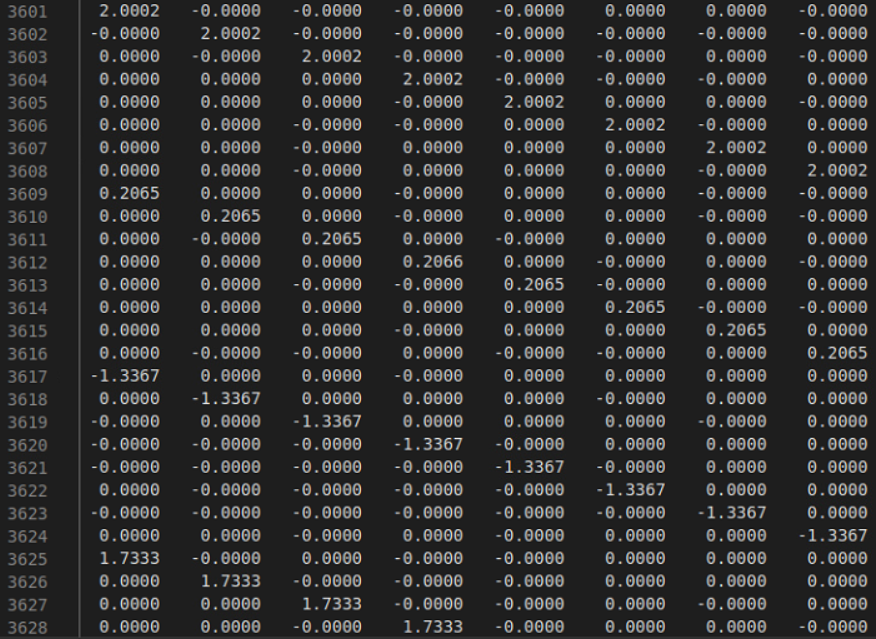
\includegraphics[width = \textwidth]{pilot8.png}
	\caption{导频实部(8 Stream)}
	\end{minipage}
	\begin{minipage}[t]{0.5\linewidth}
	\centering
	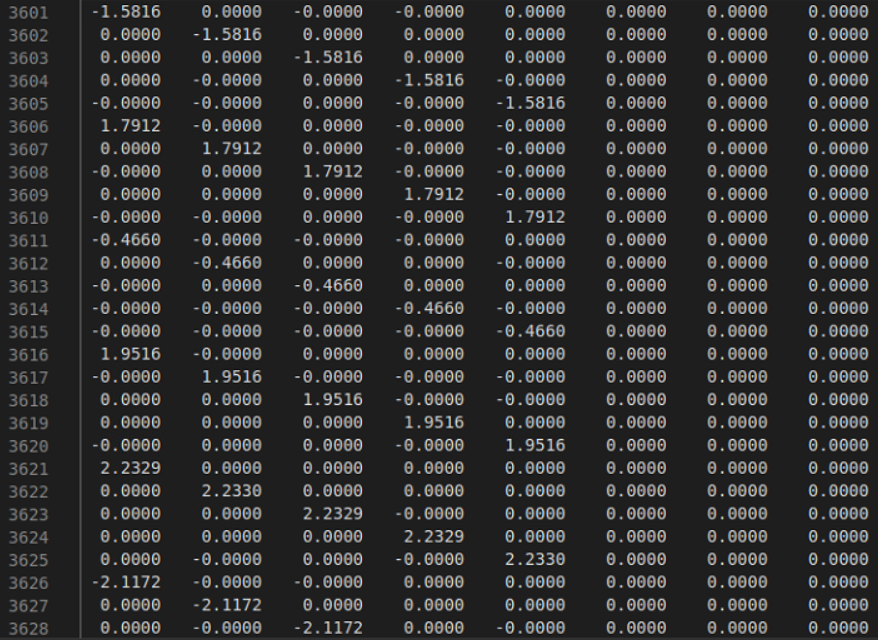
\includegraphics[width = \textwidth]{pilot5.png}
	\caption{导频实部(5 Stream)}
	\end{minipage}
\end{figure}
\subsubsection{方案二:预先生成8类导频}
\lstset{language=C++}
\begin{lstlisting}
int32_t inter_freq[MAX_BEAM] = {0, 0, 0, 0, 0, 0, 0, 0};
lapack_complex_float *pilot_symb[MAX_BEAM];
for (i = 0; i < MAX_BEAM; i++)
{
	pilot_symb[i] = (lapack_complex_float *)malloc(sizeof(lapack_complex_float) * (i + 1) * CARRIER_NUM * PILOT_SYM_NUM);
	k = i + 1;
	while (CARRIER_NUM % k != 0)
		k++;
	inter_freq[i] = k;
	CalPilotSymb(i + 1, CARRIER_NUM, PILOT_SYM_NUM, USER_NUM, inter_freq[i], pilot_symb[i]);
}
\end{lstlisting}

\subsection{R=984以及R<342时的译码问题}
\begin{figure}[H]
	\centering
	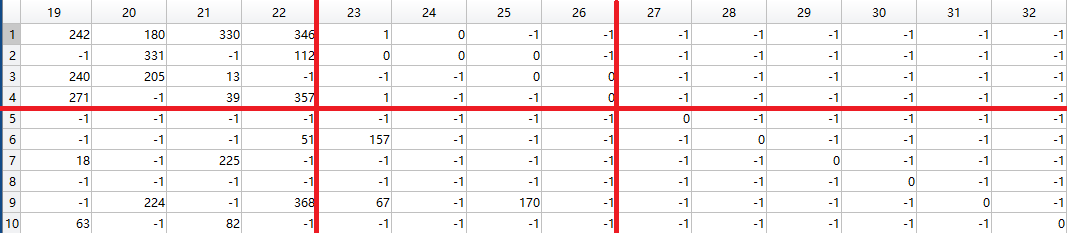
\includegraphics[width = \textwidth]{bg.png}
	\caption{BG1部分数值}
\end{figure}
\begin{lstlisting}
col_hbg_d = h->K_b * 1024 / h->R + 2;
col_hbg_d = col_hbg_d >= (h->K_b + 4) ? col_hbg_d : (h->K_b + 4);
col_hbg_d = col_hbg_d <= h->col_hbg ? col_hbg_d : h->col_hbg;
row_hbg_d = col_hbg_d - h->K_b;
\end{lstlisting}

\subsection{实现有效载波长度的可变}
\begin{figure}[H]
	\centering
	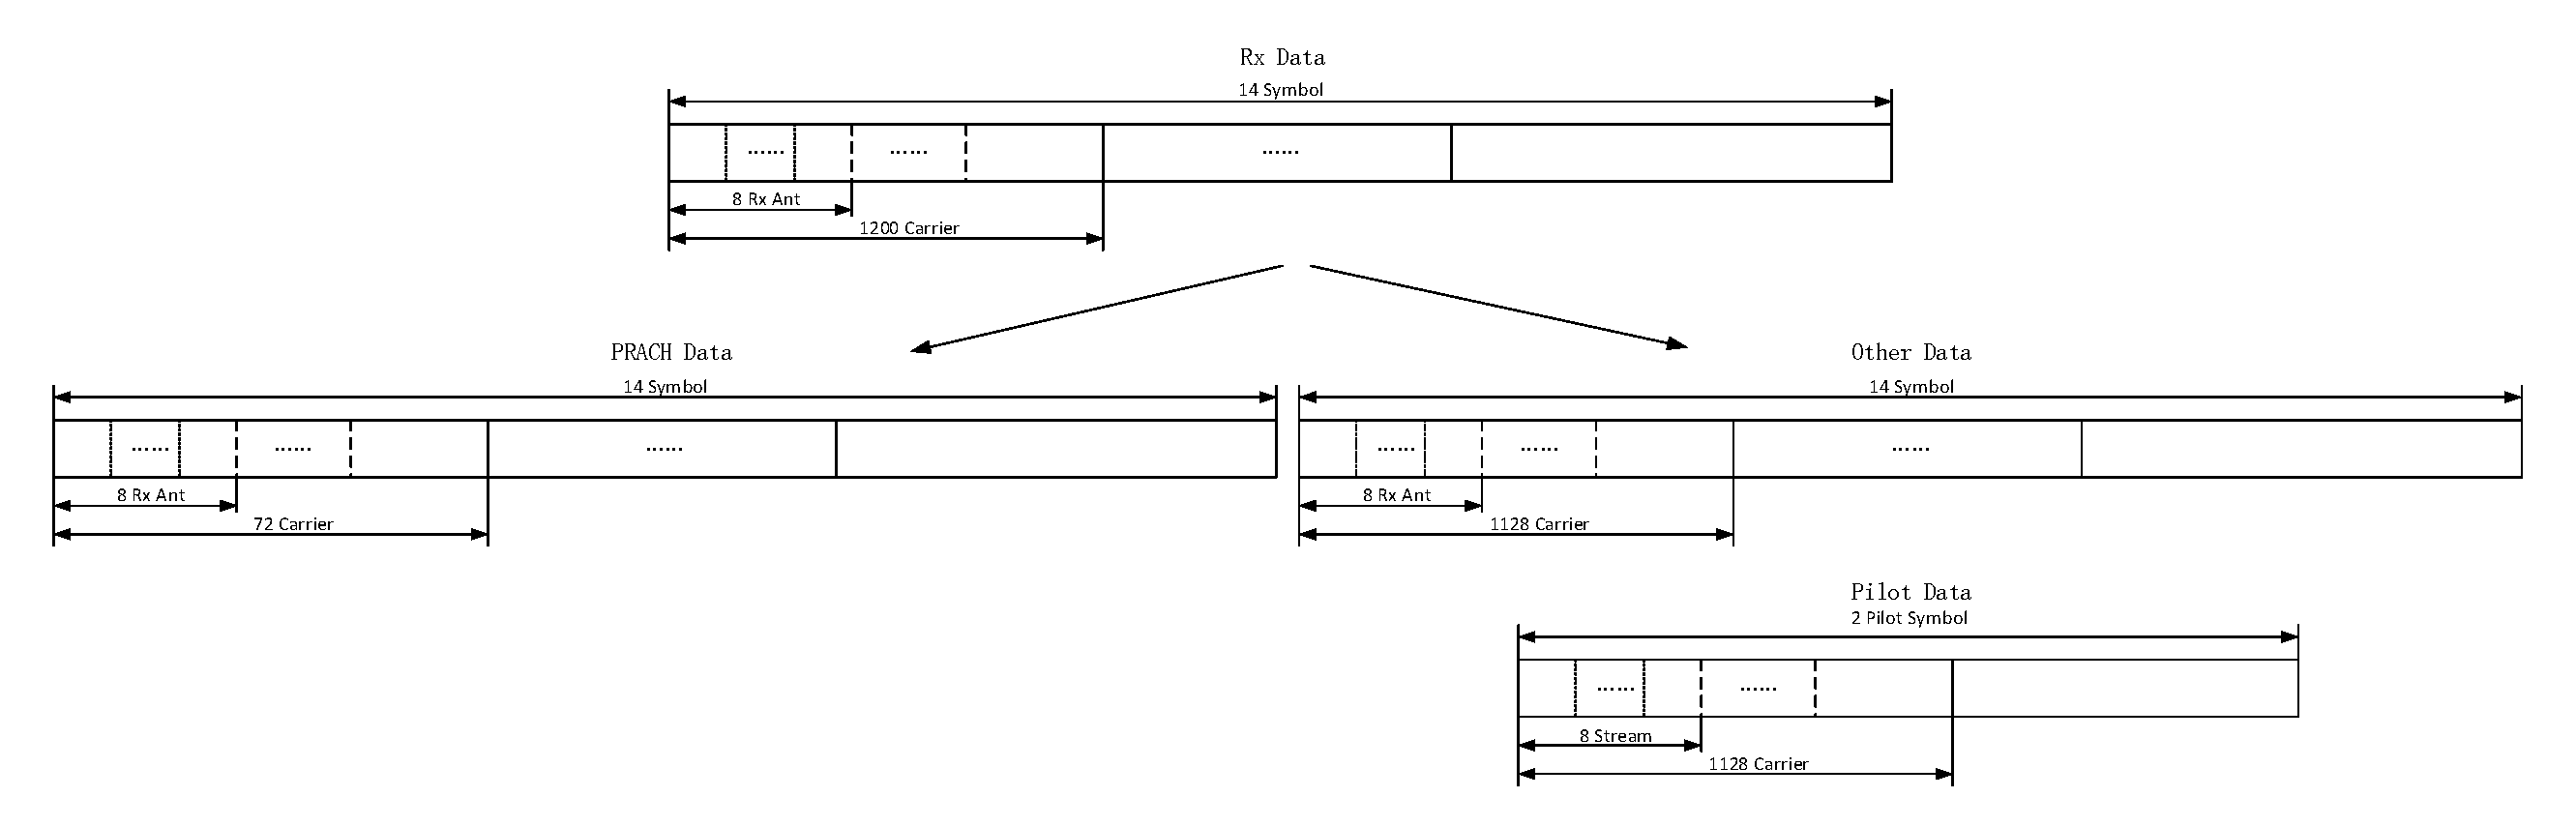
\includegraphics[width = \textwidth]{rxdata.pdf}
	\caption{Rx端数据子帧结构}
\end{figure}
\begin{lstlisting}
const int32_t vld_carrier_num_table[VLD_CARRIER_TYPE_NUM] = {1200, 1128};
......
int32_t inter_freq[VLD_CARRIER_TYPE_NUM][MAX_BEAM] = {{0, 0, 0, 0, 0, 0, 0, 0},{0, 0, 0, 0, 0, 0, 0, 0}};
lapack_complex_float *pilot_symb[VLD_CARRIER_TYPE_NUM][MAX_BEAM];
for (i = 0; i < MAX_BEAM; i++)
	for (j = 0; j < VLD_CARRIER_TYPE_NUM; j++)
	{
		pilot_symb[j][i] = (lapack_complex_float *)malloc(sizeof(lapack_complex_float) * (i + 1) * CARRIER_NUM * PILOT_SYM_NUM);
		k = i + 1;
		while (vld_carrier_num_table[j] % k != 0)
			k++;
		inter_freq[j][i] = k;
		CalPilotSymb(i + 1, vld_carrier_num_table[j], PILOT_SYM_NUM, USER_NUM, inter_freq[j][i], pilot_symb[j][i]);
	}
\end{lstlisting}

\subsection{其他改进}
1. 选择新的随机数生成方式;			\\
2. 使用fread代替fscanf读取信道信息;\\
3. 增加最大许可TBS生成模块;		\\

\subsection{当前测试接口}
\begin{lstlisting}
int32_t testNum = 8;
int32_t loopNum = 100;

float snr_list[MAX_TEST_TIMES] = {15.0, 15.0, 15.0, 15.0, 15.0, 15.0, 15.0, 15.0};
int32_t cqi_list[MAX_TEST_TIMES] = {20, 21, 22, 23, 24, 25, 26, 27};
int32_t tb_byte_len_list[MAX_TEST_TIMES] = {9162, 18327, 27492, 36657, 45823, 54988, 64153, 73318};
int32_t subcarrier_indx_list[MAX_TEST_TIMES] = {2, 3, 4, 2, 3, 4, 2, 3};
int32_t max_layer_num_list[MAX_TEST_TIMES] = {1, 2, 3, 4, 5, 6, 7, 8};	
\end{lstlisting}

%===========第二节=================
\section{性能测试}
\subsection{Tx单流耗时占比测试}
\begin{table}[H]
	\caption{Tx耗时占比}
	\centering
	\begin{tabular}{|l|l|l|l|l|}% 通过添加 | 来表示是否需要绘制竖线
		\hline  % 在表格最上方绘制横线
		Stream				& 1			& 8			\\
		\hline
		CRC Attach			& 7.64\%	& 9.65\%	\\
		\hline
		Code Blocks Segment	& 0.95\%	& 2.48\%	\\
		\hline
		Encode				& 17.89\%	& 23.31\%	\\
		\hline
		Rate Matching		& 38.31\%	& 42.39\%	\\
		\hline
		Map					& 16.33\%	& 16.25\%	\\
		\hline
		Pack				& 18.85\%	& 5.90\%	\\
		\hline  % 在表格最下方绘制横线
	\end{tabular}
\end{table}
Throuput\_Tx(Stream=1) = 94.32Mbps\\
Throuput\_Tx(Stream=8) = 126.68Mbps

\subsection{Rx单流耗时占比测试}
\begin{table}[H]
	\caption{Rx耗时占比}
	\centering
	\begin{tabular}{|l|l|l|l|l|}% 通过添加 | 来表示是否需要绘制竖线
		\hline  % 在表格最上方绘制横线
		Stream				& 1			& 8			\\
		\hline
		Channel Estimate	& 34.34\%	& 12.86\%	\\
		\hline
		Signal Detect		& 10.98\%	& 52.74\%	\\
		\hline
		Unpack				& 8.68\%	& 1.52\%	\\
		\hline
		Demap				& 9.23\%	& 10.19\%	\\
		\hline
		Rate De-matching	& 14.35\%	& 10.70\%	\\
		\hline
		Decode				& 22.18\%	& 11.67\%	\\
		\hline
		De-CBS				& 0.23\%	& 0.30\%	\\
		\hline
		CRC Check			& 2.54\%	& 1.74\%	\\
		\hline  % 在表格最下方绘制横线
	\end{tabular}
\end{table}
Throuput\_Rx(Stream=1) = 34.70Mbps \\
Throuput\_Rx(Stream=8) = 24.00Mbps

\subsection{不同流的最大吞吐量对比}
\begin{table}[H]
	\caption{最大吞吐量对比}
	\centering
	\begin{tabular}{|l|l|l|l|l|}% 通过添加 | 来表示是否需要绘制竖线
		\hline  % 在表格最上方绘制横线
		Stream	& Tx		& Rx		\\
		\hline
		1		& 94.3187Mbps	& 34.6968Mbps	\\
		\hline
		2		& 110.1581Mbps	& 21.1701Mbps	\\
		\hline
		3		& 117.0514Mbps	& 23.6051Mbps	\\
		\hline
		4		& 119.7418Mbps	& 24.6373Mbps	\\
		\hline
		5		& 124.8383Mbps	& 25.7432Mbps	\\
		\hline
		6		& 120.0644Mbps	& 23.9620Mbps	\\
		\hline
		7		& 125.5944Mbps	& 24.0412Mbps	\\
		\hline
		8		& 126.6790Mbps	& 24.0002Mbps	\\
		\hline  % 在表格最下方绘制横线
	\end{tabular}
\end{table}

\subsection{不同CQI下的性能对比}
\begin{table}[H]
	\caption{不同CQI下的性能对比(SNR=15dB, Stream=8)}
	\centering
	\begin{tabular}{|l|l|l|l|l|l|l|}% 通过添加 | 来表示是否需要绘制竖线
		\hline  % 在表格最上方绘制横线
		CQI		& Q		& R		& Tx Throughput	& Rx Throughput	& BER					& FER				\\
		\hline
		0		& 2		& 120	& 19.1748Mbps	& 1.2977Mbps	& 0.00e+00(0/2472000)	& 0.00e+00(0/100)	\\
		\hline
		1		& 2		& 157	& 24.8647Mbps	& 1.6720Mbps	& 3.09e-07(1/3235200)	& 1.00e-02(1/100)	\\
		\hline
		2		& 2		& 193	& 30.3081Mbps	& 2.0258Mbps	& 1.01e-06(4/3977600)	& 4.00e-02(4/100)	\\
		\hline
		3		& 2		& 251	& 38.0779Mbps	& 2.6368Mbps	& 1.55e-06(8/5174400)	& 8.00e-02(8/100)	\\
		\hline
		4		& 2		& 308	& 44.8342Mbps	& 3.1302Mbps	& 3.15e-07(2/6349600)	& 2.00e-02(2/100)	\\
		\hline
		5		& 2		& 379	& 53.1400Mbps	& 3.8364Mbps	& 2.30e-06(18/7814400)	& 1.60e-01(16/100)	\\
		\hline
		6		& 2		& 449	& 62.0329Mbps	& 4.5721Mbps	& 7.56e-07(7/9257600)	& 5.00e-02(5/100)	\\
		\hline
		7		& 2		& 586	& 69.5904Mbps	& 5.3592Mbps	& 5.21e-04(5648/10845600)	& 3.60e-01(36/100)	\\
		\hline
		8		& 2		& 602	& 76.7437Mbps	& 6.1579Mbps	& 1.22e-02(151672/12413600)	& 8.10e-01(81/100)	\\
		\hline
		9		& 2		& 679	& 83.4890Mbps	& 6.9832Mbps	& 7.36e-02(1030578/14001600)	& 1.00e+00(100/100)	\\
		\hline
		10		& 4		& 340	& 55.8664Mbps	& 5.9989Mbps	& 1.23e-03(17220/14022400)	& 3.50e-01(35/100)	\\
		\hline
		11		& 4		& 378	& 60.4923Mbps	& 6.6838Mbps	& 4.62e-06(72/15589600)	& 5.00e-01(50/100)	\\
		\hline
		12		& 4		& 434	& 67.1290Mbps	& 7.6519Mbps	& 1.49e-02(266314/17900000)	& 7.90e-01(79/100)	\\
		\hline
		13		& 4		& 490	& 74.0037Mbps	& 8.7083Mbps	& 2.21e-01(4471324/20209600)	& 1.00e+00(100/100)	\\
		\hline
		14		& 4		& 553	& 79.8351Mbps	& 9.7716Mbps	& 2.07e-01(4718078/22808800)	& 1.00e+00(100/100)	\\
		\hline
		15		& 4		& 616	& 87.1937Mbps	& 10.9847Mbps	& 1.46e-01(3714578/25407200)	& 1.00e+00(100/100)	\\
		\hline
		16		& 4		& 658	& 91.3331Mbps	& 11.7369Mbps	& 1.23e-01(3350474/27140000)	& 1.00e+00(100/100)	\\
		\hline
		17		& 6		& 438	& 72.5977Mbps	& 10.1401Mbps	& 2.45e-01(6644275/27098400)	& 1.00e+00(100/100)	\\
		\hline
		18		& 6		& 466	& 76.2555Mbps	& 10.7902Mbps	& 2.23e-01(6430297/28831200)	& 1.00e+00(100/100)	\\
		\hline
		19		& 6		& 517	& 83.7652Mbps	& 12.2214Mbps	& 2.05e-01(6543188/31986400)	& 1.00e+00(100/100)	\\
		\hline
		20		& 6		& 567	& 89.6400Mbps	& 13.3132Mbps	& 1.98e-01(6933854/35080000)	& 1.00e+00(100/100)	\\
		\hline
		21		& 6		& 616	& 94.9979Mbps	& 14.5417Mbps	& 1.93e-01(7371623/38112000)	& 1.00e+00(100/100)	\\
		\hline
		22		& 6		& 666	& 101.6158Mbps	& 15.9313Mbps	& 1.97e-01(8124062/41205600)	& 1.00e+00(100/100)	\\
		\hline
		23		& 6		& 719	& 107.3590Mbps	& 17.3358Mbps	& 1.90e-01(8441999/44485600)	& 1.00e+00(100/100)	\\
		\hline
		24		& 6		& 772	& 112.6666Mbps	& 18.8440Mbps	& 1.89e-01(9018436/47764800)	& 1.00e+00(100/100)	\\
		\hline
		25		& 6		& 822	& 111.5673Mbps	& 19.2854Mbps	& 1.89e-01(9610630/50858400)	& 1.00e+00(100/100)	\\
		\hline
		26		& 6		& 873	& 108.4685Mbps	& 20.1055Mbps	& 1.93e-01(10419103/54014400)	& 1.00e+00(100/100)	\\
		\hline
		27		& 6		& 910	& 114.9944Mbps	& 21.3412Mbps	& 1.93e-01(10868537/56303200)	& 1.00e+00(100/100)	\\
		\hline
		28		& 6		& 948	& 116.7884Mbps	& 21.9075Mbps	& 1.89e-01(11105305/58654400)	& 1.00e+00(100/100)	\\
		\hline  % 在表格最下方绘制横线
	\end{tabular}
\end{table}

%===========第三节=================
% \section{根据PRACH测时延}
% \begin{figure}[H]
% 	\centering
% 	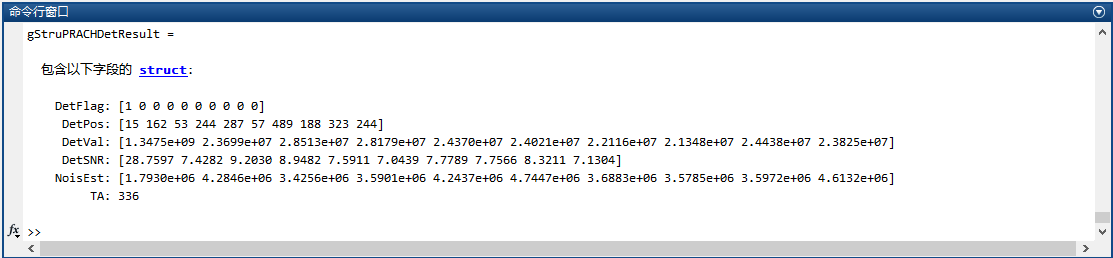
\includegraphics[width = \textwidth]{prach.png}
% 	\caption{时延测试结果}
% \end{figure}

%===========第四节=================
% \section{后续工作}
% 1. 实现当前SVN目录结构下基于LDPC的单线程编码调制链路;

%===========下周计划=================
% \section{下阶段计划}
% 1. 完善单线程系统(修复Bug)

\end{document}
%%%%%%%%%%%%%%%%%%%%%%%这是正文部分的结束%%%%%%%%%%%%